\chapter{Introduction}\label{introduction}
//TODO Write what is NLP

\chapter{Dialogue systems}\label{dialogue systems}
Dialogue system is a computer system to communicate with a human. Nowadays you meet dialog systems everywhere. A lot of devices have incorporated goal-oriented spoken dialogue systems, such as  Yandex’s Alisa,  Apple’s Siri, Microsoft’s Cortana, Amazon Alexa, and Google Assistant. Dialogue systems are also used in cars (hands-free car-specific functions, Android Auto, Apple CarPlay, vendor-specific solutions), web (search assistants (IKEA), Facebook Messenger and Telegram chatbots), robots, computer games, research systems (skylar.speech.cs.cmu.edu) etc, because a conversation is a natural way for people to get information.

\textbf{Basic Dialogue System Types}:
\begin{itemize}
  \item Task-oriented 
    \begin{itemize}
      \item focused on completing a certain task(s)
    \end{itemize}
  \item Non-task-oriented
    \begin{itemize}
      \item chitchat
      \item gaming the Turing test
    \end{itemize}    
\end{itemize}

\textbf{Communication Domains}:

"\textbf{Domain}" is a conversation topic or an area of interest
\begin{itemize}
  \item Single/Closed-domain is one well-defined area
  \item Multi-domain is joining several single-domain systems
  \item Open-domain “responds to anything”
\end{itemize}


Exists several \textbf{modes of communication}:
\begin{itemize}
  \item Text
  \item Voice
  \item Multimodal
    \begin{itemize}
      \item voice/text + graphics
      \item additional modalities: video - gestures, mimics; touch
    \end{itemize}
\end{itemize}

\textbf{Dialogue initiative}:
\begin{itemize}
  \item system-initiative
    \begin{itemize}
      \item system asks questions, user must reply in oreder to progress
      \item least natural
      \item "form-filling" ("Hello, please enter your e-mail") 
    \end{itemize}
  \item user-initiative
    \begin{itemize}
      \item user asks, machine responds ("Siri, set the timer for 5 minutes")
    \end{itemize}
  \item mixed-initiative
    \begin{itemize}
      \item system and user both can ask and react to queries
      \item most natural
    \end{itemize}
\end{itemize}

\textbf{Dialogue system architecture} is illustrated in Figure \ref{ds architecture}. This architecture consists from Natural Language Understanding (NLU), dialogue management (DM), and Natural Language Generation (NLG).

\textbf{NLU} extracts the meaning from the user utterance and converts into a structured semantic representation. Natural Language Understanding traditionally consists of domain identification and intent prediction, which are framed as utterance classification problems, and slot filling, framed as a sequence tagging task.

\textbf{DM} plays two roles,tracking the dialogue state and performing the dialogue policy (i.e., telling the agent how to act given the dialogue state.)

\textbf{NLG} transforms structured data into natural language.\cite{open_domain_neural_ds}
\begin{figure}[hbt]
  \centering
  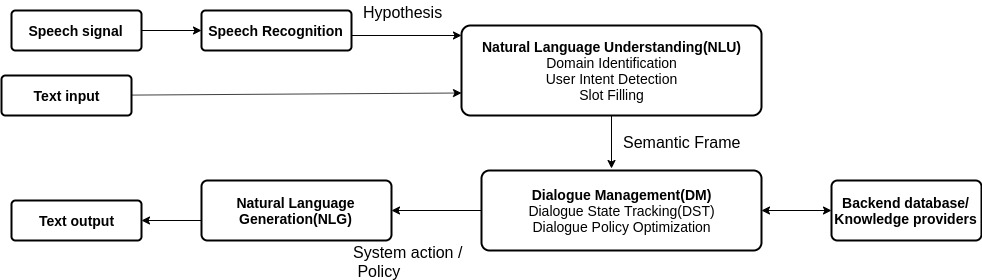
\includegraphics[width=0.8\textwidth]{figures/ds_arcitecture.jpg}
  \caption{Dialogue system architecture.}
  \label{ds architecture}
\end{figure}

\chapter{Natural Language Generation}\label{nlg}
Natural Language Generation is a subsection of Natural Language Processing (NLP). NLG uses different methods and tricks to convert data to human language.

\section{Architecture of NLG}
  Reiter and Dale in the article \cite{applied_nlg} proposed architecture splitted into 3 stages, which is illustrated in Figure \ref{nlg architecture}. 
\begin{figure}[hbt]
  \centering
  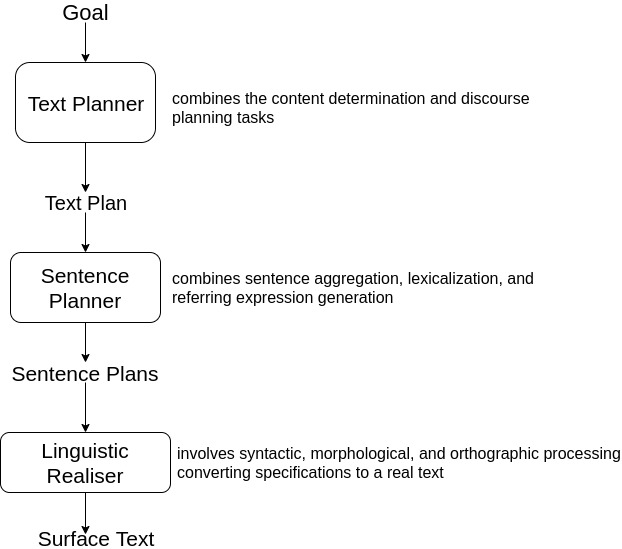
\includegraphics[width=0.7\textwidth]{figures/nlg_architecture.jpg}
  \caption{NLG architecture.}
  \label{nlg architecture}
\end{figure}

This pipeline shows the milestones of natural language generation, however, specific steps and approaches, as well as the models used, can vary significantly with the technology development.

NLG approaches can be grouped into two categories, one focuses on generating text using templates or rules (linguistic) methods, the other uses corpus-based statistical/dynamic methods, where \textbf{corpus} is a collection of texts.

\section{Categories of Natural Language Generation approaches}

\subsection{Template-based approach} 
Template-based systems map their non-linguistic input directly to the linguistic surface structure. This linguistic structure may contain gaps. Well-formed outputs does not cointain gaps.
The template-based system selects a proper response for the current conversation from a repository with response selection algorithms. 

This approach has a long development way from simple gap-filling to word-level grammatical functions:

\textbf{Gap-Filling Approach} is one of the oldest approaches, that can automatically fill gaps in text, that have a predefined structure, with a small amount of data retrieved from a spreadsheet row, database table entry, etc. This approach is a quite limited.

\textbf{Scripts or Rules-Producing Text} is an approach, that expands basic gap-filling systems with general-purpose programming constructs via a scripting language or by using business rules. These systems still lack linguistic capabilities and cannot generate high-quality text reliably.

\textbf{Word-Level Grammatical Functions} was adding to template-based systems to deal with morphology, morphophonology and orthography. These functions made it easier to generate grammatically correct texts and to write complex template systems.

\subsubsection{Advantages of template-based systems}
Template-based systems have a number of advantages: the output produced by this approach is likely to be grammatically correct and not contain unexpected generation errors; process of sentence generation is fully controlled; these models are robust and reliable because they consist of clearly defined rules.

\subsubsection{Disadvantages of template-based systems}
Despite all the above, template-based approach has some disadvantages. First of all, this models requires time and human resources to deploy a real dialogue system, because templates are constructed manually, and the number of templates grows quickly (using different templates for singular and plural versions); these systems are not able to handle unknown inputs; templates often sound unnatural due to their generic structures; template-based systems cannot make variation in output, it is just concatenation of strings; this approach is not flexible, because it has limits to use templates in other domains; and finally a template-based model is not able to learn and is not able to adapt to the user.

\begin{center}
\subsubsection{Example}\label{tb_example} 
"The 306 train leaves Aberdeen at 11:20 am"

\vspace{5mm}
Semantic representation: 

$Departure(train_{306}, location_{abdn}, time_{1120})$

\vspace{5mm}
Template: 

[train] \textit{is leaving} [town] \textit{now}
\end{center}

The gaps represented by \textbf{[train]} and \textbf{[town]} are filled by looking up the relevant
information in a table. More information you can find in \cite{applied_nlg}.

\subsection{Corpus-based/Dynamic approach}
Corpus-based dominates the NLG community, special in the case of open-domain tasks, where it is almost impossible to hand-craft the templates for all possible combinations of semantic units and their respective surface realization.
In corpus-based systems include statistical and machine learning approaches. 

One of the first approaches in corpus-based methods was \textbf{Dynamic Sentence Generation}, that dynamically creates sentences from representations of the meaning to be conveyed by the sentence and/or its desired linguistic structure. It allows do not write code for every boundary case and includes aggregation, reference, ordering and connectives to optimise sentences.

Next level of corpus-based approaches was \textbf{Dynamic Document Creation}, what can produce relevant and well-structured document. 

\subsubsection{Advantages of corpus-based approach}
Corpus-based models have some advantages: they have ability to generate more proper responses that could have never appeared in the corpus; it is possible to mimick the language of a real domain expert and use this models for open-domain dialogue systems; dynamic approach is able to learn and to handle unknown inputs, it is also has a lot of possible varioations of output.

\subsubsection{Disadvantages of corpus-based approach}
Unfortunately corpus-based systems have some disadvantages. It is necessary to have a good corpus, it should contain a large amount of data and on a variety of topics to get a sensible output. Even if you have a good corpus, process of text generation is not fully controlled and the output can be grammatically incorrect.

More information you can find in \cite{stochastic_language_generation_ds} \cite{survey_on_ds} \cite{data_driven_nlg}.

\section{Model components for Natural Language Generation}
NLG evolution from templates to dynamic generation of sentences took a lot of time and models developed along with it. Corpus-based generation uses a generative probabilistic model what can be implemented in many ways.

One of the first model's implementation was \textbf{Markov chain}. It is a stochastic model, that is used to describe the next event in a sequence given the previous event only by probabilistic weighting. It does not track all the previous states in a sequence to conclude what is the next possible state. In our case state is an n-gram(contiguous sequence of n items from text or speech).

The next model, what is used in NLG, is \textbf{Recurrent neural network (RNN)}. Neural networks are computing systems that are inspired by biological neural networks. A "neuron" is a mathematical function that classifies and collects information according to a specific architecture. A neural network contains layers of interconnected "neurons". RNN takes series of input with no predetermined limit on size. Recurrent neural network passes each item of the sequence through a feedforward network and stores the information from the previous step. In each iteration this model calculates the probability of the next item with using information in the memory.

The architecture of RNN is illustrated in Figure \ref{rnn}, where coefficient \textbf{h} is a hidden layer, \textbf{x} is an input and \textbf{y} is an output. Coefficient \textbf{w} is a weight, what is transformed to produce a sensible output.

The RNN-based models have been used for NLG as an end-to-end training network \cite{network_nlg} and a training model with semantic aggregation \cite{rnn_nlg}. 

Nowadays RNN networks almost are not used in NLG, because it has problems with vanishing and exploding gradient. The long-term information travels sequentially  through all cells before getting to the present processing cell. This means, that it can be easily corrupted by being multiplied many time by small or big numbers. Other problem of RNN is that they are not hardware friendly, it takes a lot of resources to train and run this network. More information about difficulties of training RNN you can find in \cite{rnn_difficulties}.

\begin{figure}[hbt]
  \centering
  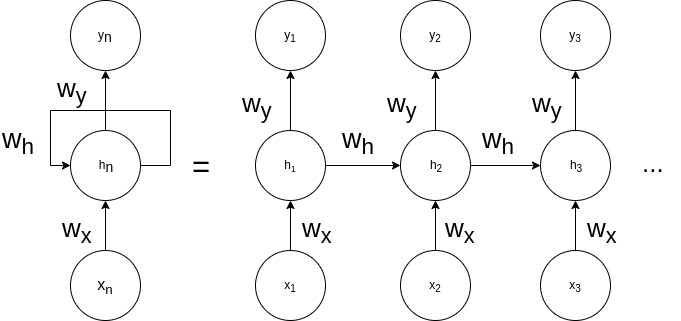
\includegraphics[width=0.5\textwidth]{figures/rnn.jpg}
  \caption{Architecture of recurrent neural network.}
  \label{rnn}
\end{figure}


\textbf{LSTM} networks are a special kind of RNN, capable of learning long-term dependencies. All recurrent neural networks have the form of a chain of repeating modules of neural network. LSTM network also has this chain structure, but the repeating module has a different structure. 

In Figure \ref{lstm} each line carries an entire vector from the output of one node to the inputs of others. The circles represent pointwise operations, while rectangles are learned neural network layers. Lines merging denote concatenation, while a line forking denote its content being copied and the copies going to different locations.

This model resolved a problem with vanishing gradient, but still the capacity of the LSTM memory is limited, because of inherently complex sequential words' paths from the previous unit to the current unit. The same complexity results in high computational requirements that make LSTM difficult to train or parallelize.

\begin{figure}[hbt]
  \centering
  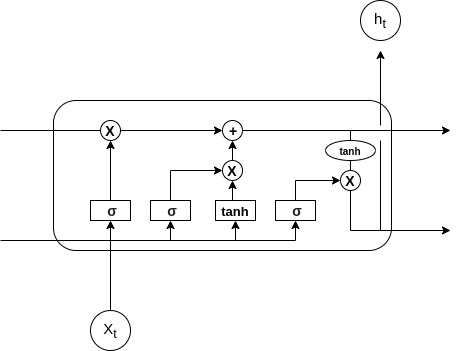
\includegraphics[width=0.3\textwidth]{figures/lstm.jpg}
  \caption{A cell in an LSTM network.}
  \label{lstm}
\end{figure}


\textbf{Transformer} is a relatively new architecture, which proposes a "self-attention mechanism". This model was introduced in the paper "Attention is all you need" \cite{transformer} in 2017. The advantage of this model is a constant number of operations, which simplifies the parallelization of processes. The Transformer uses the representation of all words in context without compressing all information into a single fixed-length representation that allows the system to handle longer sentences without the skyrocketing of computational requirements. 

The architecture of the Transformer is illustrated in Figure \ref{transformer}. The Transformer consists of a stack of encoders (on the left) for processing inputs of any length and another set of decoders (on the right) to output the generated sentences. The inputs and output are first embedded into an n-dimensional space since we cannot use strings directly. The Transformer cannot remember how sequences are fed into a model, because of it positions are added to the embedded representation (n-dimensional vector) of each word.

\begin{figure}[hbt]
  \centering
  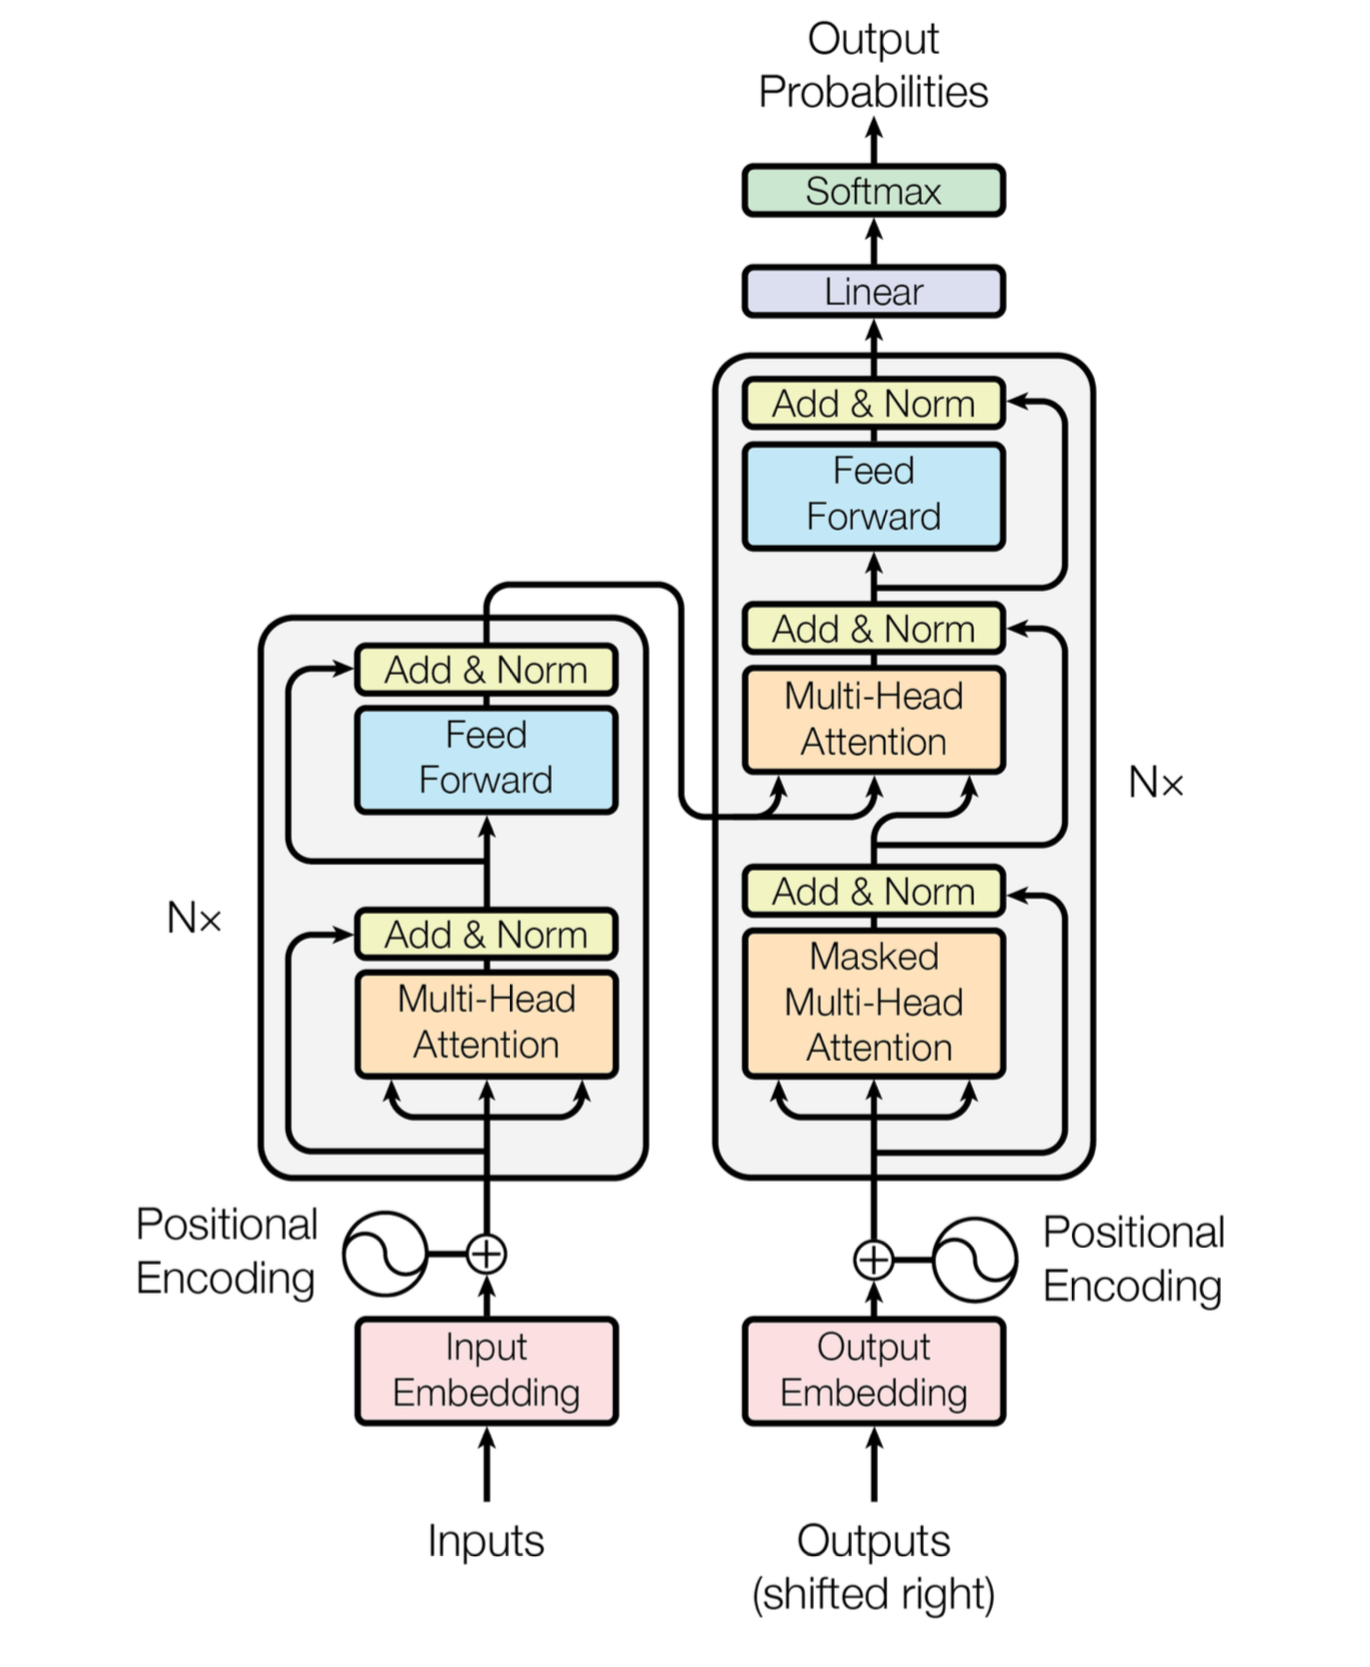
\includegraphics[width=0.5\textwidth]{figures/transformer.png}
  \caption{The architecture of the Transformer\cite{transformer}}
  \label{transformer}
\end{figure}

\subsection*{NLG problems}
The NLG component converts an abstract dialogue action into natural language surface utterances. In NLG it is necessary to control not only correctness of output but also if output is appropriate or felicitous in a given context. As noticed in \cite{generator_problems}, a good generator usually relies on several factors: adequacy (similarity in meaning), fluency (syntactic correctness), readability (efficacy in context), and variation.

\chapter{Other}
Oh and Rudnicky showed that stochastic generation benefits from two factors: 
\begin{itemize}
  \item it takes advantage of the practical language of a domain expert instead of the developer
  \item it restates the problem in terms of classification and labeling, where expertise is not required for developing a rule-based generation system
\end{itemize}

Non-task-oriented dialogue system

The aim of task-oriented dialogue systems is to complete specific tasks fo user, non-task-oriented dialogue systems focus on conversing with human on open domains. 

//TODO: more information in article []
//TODO: Info about datasets
//TODO: NLP vs Computation linguistic

//TODO: In non task oriented dialogue systems it is very difficult to use template-based generation
\cite{stochastic_language_generation_ds}
